% Day 4: why action needs a second functional. \input from day4.tex.
% Frames moved from Day 1 on 2026-10-17. Figures d1_candidates.pdf / d1_diminishing.pdf are produced
% by figures/make_day1.py; d4_* by figures/make_day4.py.

% =================================================================================================
\section{Why action needs a second functional}
% =================================================================================================

\begin{frame}{Monday's frame, now done properly}
  \begin{columns}[c]
    \begin{column}{0.5\textwidth}
      \centering
      \begin{tikzpicture}[x=2.3cm, y=1.5cm, lab/.style={font=\scriptsize}]
        \draw[-{Stealth}, muted] (0,0) -- (2.15,0) node[below left, lab, text=black] {action $a$};
        \draw[-{Stealth}, muted] (0,0) -- (0,1.45) node[right, lab, text=black] {nats};
        \draw[accent, very thick] (0,0.75) -- (2.05,0.75);
        \node[lab, below] at (1.62,0.75) {$F[q,o_t]$: flat};
        \visible<2->{
        \draw[cool, very thick, domain=0:2.05, samples=50] plot (\x, {0.2 + 0.72*(\x-1.2)*(\x-1.2)});
        \fill[cool] (1.2,0.2) circle (2pt);
        \node[lab, above right] at (1.2,0.28) {$a^\ast$};
        \node[lab, align=center] at (1.42,1.2) {$\E[F]$ of what\\$a$ would bring};}
      \end{tikzpicture}
    \end{column}
    \begin{column}{0.46\textwidth}
      \textbf{Perception.} $o_t$ is fixed, so only $q$ can move.

      \vspace{0.6em}
      \textbf{Action.} At decision time $o_t$ is a number in a buffer:
      \[ \frac{\partial F[q,o_t]}{\partial a} = 0 . \]
      \pause
      What action \emph{can} change is the free energy of data not yet received:
      \[ a^\ast = \argmin_a \E_{q(o_{t+1},s_{t+1}\given a)}\big[F[q,o_{t+1}]\big] \]
    \end{column}
  \end{columns}
  \src{active\_inference.tex l.335--369}
\end{frame}

\begin{frame}{Expected free energy}
  For a policy $\pi$, with predicted states and observations $\tilde s,\tilde o$, and goals entering
  as a \textbf{prior over preferred outcomes} $p(\tilde o)$:
  \[ G(\pi) = \E_{q(\tilde s,\tilde o\given\pi)}\big[\ln q(\tilde s\given\pi) - \ln p(\tilde o,\tilde s)\big] \]
  Add and subtract $\ln q(\tilde s\given\tilde o,\pi)$, and split the joint. Exactly:
  \[
    G(\pi) = \E\Big[
      \underbrace{\ln q(\tilde s\given\pi) - \ln q(\tilde s\given\tilde o,\pi)}_{\text{epistemic}}
      \;\underbrace{-\ln p(\tilde o)}_{\text{pragmatic}}
      + \underbrace{\ln q(\tilde s\given\tilde o,\pi)-\ln p(\tilde s\given\tilde o)}_{\to 0 \text{ if inference stays good}}
    \Big]
  \]
  \lesson{No reward channel, no separate exploration bonus: both come out of the same line.}
  \src{active\_inference.tex l.371--412}
\end{frame}

\begin{frame}{Two terms, one currency}
  \centering
  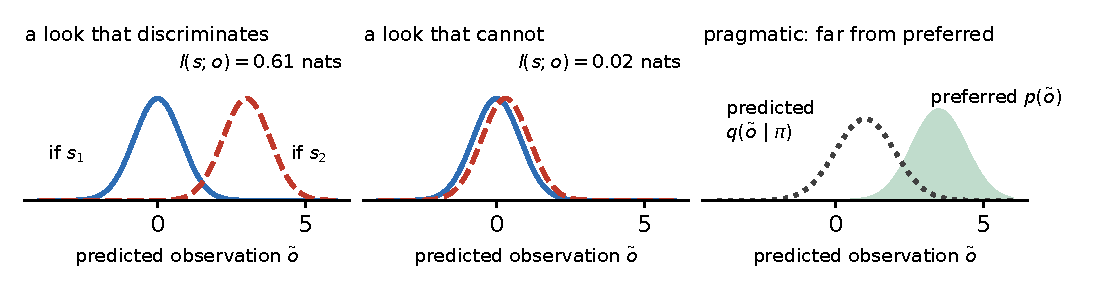
\includegraphics[width=0.97\textwidth]{d4_terms.pdf}

  \vspace{0.3em}
  \begin{columns}[T]
    \begin{column}{0.62\textwidth}
      \small
      \textbf{Epistemic} $=-I(\tilde s;\tilde o\given\pi)$: largest when what you would see depends on
      what is true.
    \end{column}
    \begin{column}{0.34\textwidth}
      \small
      \textbf{Pragmatic} $=-\E\ln p(\tilde o)$: what a cost function would have held.
    \end{column}
  \end{columns}

  \vspace{0.5em}
  \lesson{Both are in nats, derived together. The balance moves as the beliefs sharpen.}
  \src{active\_inference.tex l.414--427; curves: figures/make\_day4.py, block 1}
\end{frame}

\begin{frame}{For Gaussian beliefs, three names for one number}
  \begin{columns}[c]
    \begin{column}{0.36\textwidth}
      \centering
      \begin{tikzpicture}
        \draw[cool, very thick, rotate=25] (0,0) ellipse (1.7cm and 0.95cm);
        \draw[accent, very thick, rotate=70, fill=accent!25] (0,0) ellipse (0.85cm and 0.42cm);
        \node[font=\scriptsize, text=cool] at (0.15,1.25) {$\Lambda$: before};
        \node[font=\scriptsize] at (0,-1.45) {$\Lambda + J^\top R^{-1}J$: after};
      \end{tikzpicture}\\[0.3em]
      {\small $\Delta H$ is the log of the area ratio.}
    \end{column}
    \begin{column}{0.6\textwidth}
      \[
        \underbrace{H[q]-\E H[q\given o]}_{\text{expected entropy drop}}
        = \underbrace{I(s;o)}_{\text{mutual information}}
      \]
      \[
        = \underbrace{\tfrac12\ln\frac{|\Lambda + J^\top R^{-1}J|}{|\Lambda|}}_{\text{D-optimal design}}
      \]
      \small
      The epistemic term, the information gain of active sensing and the criterion of optimal
      experiment design are \alert{one quantity}. It depends on \emph{where} you look, not on
      \emph{what} you will see, so it can be computed before moving.
    \end{column}
  \end{columns}
  \src{appendix\_math.tex l.742--779, l.1236--1287}
\end{frame}

\begin{frame}{Where to look next}
  \begin{columns}[c]
    \begin{column}{0.58\textwidth}
      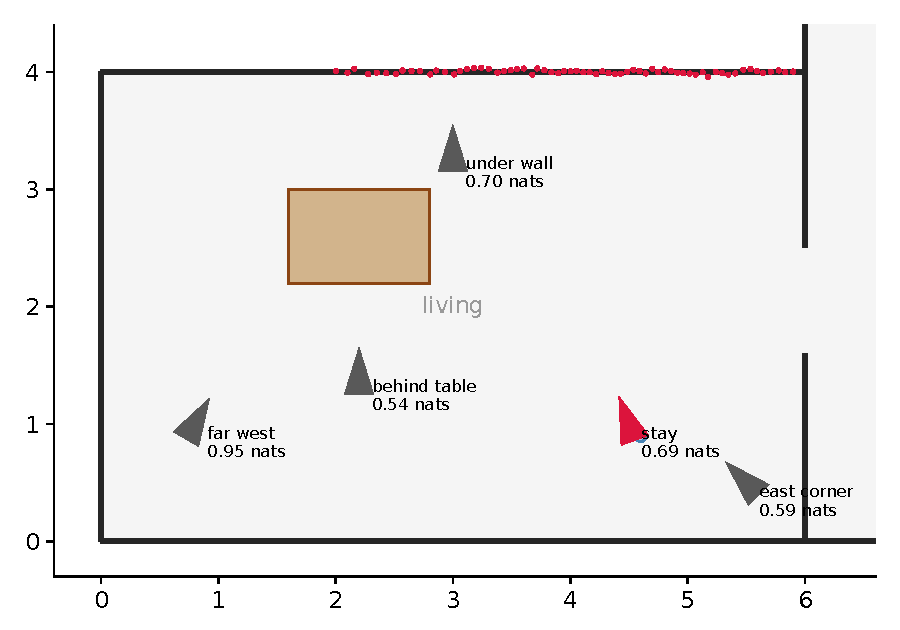
\includegraphics[width=\textwidth]{d1_candidates.pdf}
    \end{column}
    \begin{column}{0.4\textwidth}
      \small
      Monday's wall: the robot (red) has seen its east part. Five candidate viewpoints.
      \begin{itemize}
        \item ``far west'' sees few points and gains the most: it adds lever arm where the
              information is weak;
        \item ``stay'' gains exactly $\ln 2$. Why?
      \end{itemize}
    \end{column}
  \end{columns}
  \src{lab 4, exercise 1}
\end{frame}

\begin{frame}{Diminishing returns, and a warning}
  \begin{columns}[c]
    \begin{column}{0.45\textwidth}
      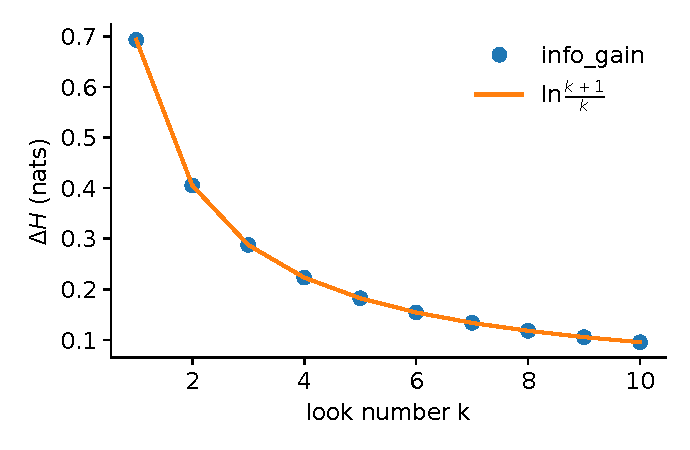
\includegraphics[width=\textwidth]{d1_diminishing.pdf}
    \end{column}
    \begin{column}{0.53\textwidth}
      \small
      The $k$-th identical look gives $|(k{+}1)\Lambda_1| / |k\Lambda_1|=((k{+}1)/k)^2$ for two
      parameters, so
      \[ \Delta H_k = \ln\frac{k+1}{k}. \]
      \pause
      \alert{But this assumes each look's errors are independent.} Repeated looks share the pose
      and the calibration, and those do not average away.\\[0.4em]
      Day 3's common-mode ceiling already put a number on how little a repeat look is worth.
    \end{column}
  \end{columns}
  \src{lab 4, exercise 2}
\end{frame}
